\chapter{Magnitude and shape distributions for mock selection of DESI targets}

\section{DESI Target selection}

%https://doi.org/10.3847/1538-3881/ab089d
%https://ui.adsabs.harvard.edu/abs/2013AJ....145...10D/abstract
%https://academic.oup.com/mnras/article/455/2/1553/1112409#92067589
% CLASS = TARGET TYPE?
% What tense should this be in - past or present?
% Make comparison to eBOSS?
% Describe cuts made on the data
% Include description of each shape profile
% Include description of density contours for 2D Gaussian
% There is noticable difference between my results and John's albeit he used different cuts - could this be due to the cuts, but also because he is running the GMMs on DR 7.1? Did Tractor calculation of fluxes improve in subsequent data releases?

DESI will extract spectra from over 35 million astrophysical sources to measure the expansion rate over the past 11 billion years. To do this it will need an inventory of targets to choose from so that it can know where to point its 5,000 optical fibers. DESI pre-selected targets to observe from three separate imaging surveys, collectively referred to as the DESI Legacy Imaging Surveys. These wide-field surveys provided photometry that was both uniform and spatially dense, ultimately pushing to depths around 2 magnitudes deeper than SDSS.  Compared to SDSS, the Legacy Surveys detected over 15 times the number of $z>0.5$ galaxies and over 200 times more $z>1.0$ galaxies by reaching $5\sigma$ depth in the z-band (Dey et. al Overview). The utility of these surveys goes beyond target selection for DESI, as they can be used in tandem with overlapping spectroscopic data in a variety of contexts such as redshift estimation through the use of spectroscopic priors or to study dark matter halos by cross-correlating spectroscopic and imaging maps (Dey et. al Overview).

\subsection{DESI Legacy Imaging Surveys}

The Legacy Surveys completely overlap with DESI's approximately 14000 deg$^2$ footprint, which is divided into separate 9900 deg$^2$ and 4000 deg$^2$ patches in each of the Northern and Southern Galactic Caps, respectively (Fig. \ref{fig:footprint}). The Dark Energy Camera (DECam, Flaugher et al 2015), which is installed on the 4-meter Blanco telescope at the Cerro Tololo Inter-American Observatory, imaged the entire SGC footprint and part of the NGC in $g,r,z$ bands as part of the Dark Energy Camera Legacy Survey (DECaLS). The majority of DESI's northern footprint was imaged at Kitt Peak National Observatory. Photometry in the $g$- and $r$-bands was taken by the Prime90 instrument on the Bok Telescope as part of the Beijing-Arizona Sky Survey (BASS, Zou et al 2017b), and additional $z$-band photometry was provided by the Mayall z-band Legacy Survey (MzLS) which used the Mosaic-3 camera on the Mayall 4-meter Telescope. These optical data were combined with mid-infrared photometry from the Wide-field Infrared Survey Explorer (WISE) satellite (ref) to help differentiate between targets and characterize morphology, and were particularly useful for selecting luminous red galaxies and quasars. See Table \ref{tab:legacy} for more info about survey coverage and depths. (Might want to include Table 1 and/or Table 2 from Dey et. al)

\begin{figure}\centering
\subfloat[g-band]{\label{a}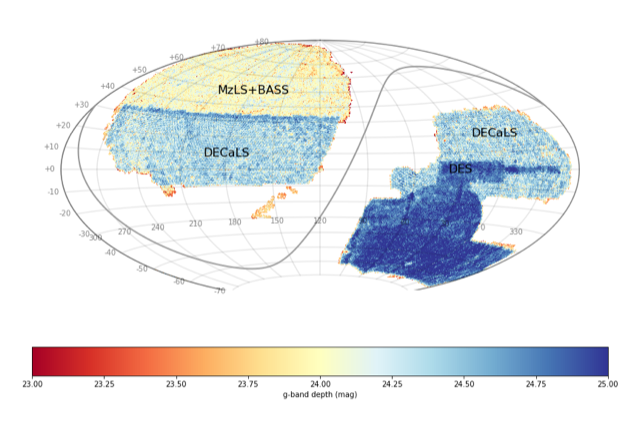
\includegraphics[width=.45\linewidth]{images/gmm/depth-g-dr9.png}}\hfill
\subfloat[r-band]{\label{b}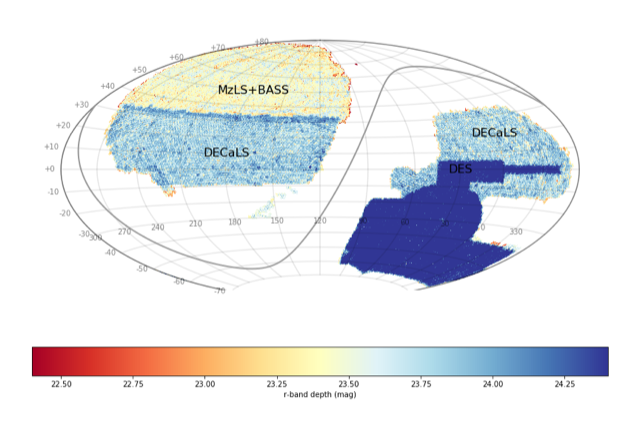
\includegraphics[width=.45\linewidth]{images/gmm/depth-r-dr9.png}}\par 
\subfloat[z-band]{\label{c}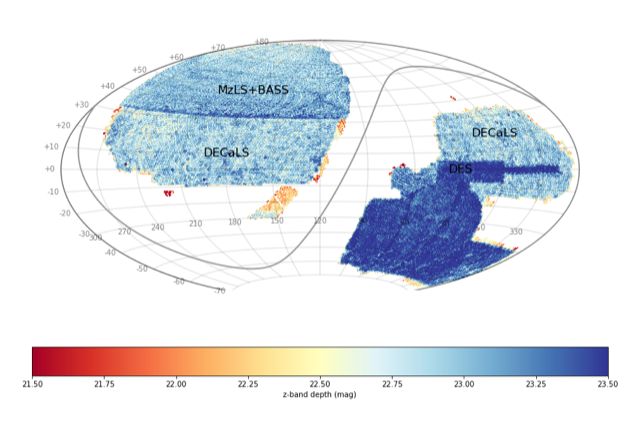
\includegraphics[width=.45\linewidth]{images/gmm/depth-z-dr9.png}}
\caption{DR9 footprint. Credit: https://www.legacysurvey.org/status/}
\label{fig:footprint}
\end{figure}


% Fix the qsos in the table so that number and z range are split for the same class
\begin{table}
\caption{DESI Legacy Surveys: Areas and Depths}
\label{tab:legacy}
\centering
\begin{tabular}{c c c c c}
\toprule
\multicolumn{4}{c}{}   \\
  Survey Name & Telescope/Instrument & Galaxy Depth (mag) & Area (deg$^2$) & Location\\
  \hline \hline
  DECaLS & Blanco/DECam & \begin{tabular}{c|c|c}
  g & r & z\\
  \hline
  23.72 & 23.27 & 22.22 \\
  \end{tabular}
  & 9000 & NGC(\delta \leq+32^{\circ})+SGC\\
  \hline
  BASS & Bok/90Prime & \begin{tabular}{c|c}
  g & r \\
  \hline
  23.48 & 22.87 &  \\
  \end{tabular} & 5000 & NGC(\delta \geq+32^{\circ})\\
  \hline
  MzLS & Mayall/Mosaic-3 & \begin{tabular}{c}
  z\\
  \hline
   &  &  22.29\\
  \end{tabular} & 5000 & NGC(\delta \leq+32^{\circ})\\
  \hline
\end{tabular}
%Median 5$\sigma$ detection limit in AB mag for the fiducial DESI target 
%Add WISE info?
\end{table}\\

\subsection{Target classes}
%sources from: https://www.desi.lbl.gov/2020/11/04/desi-target-selection/

DESI will observe luminous red galaxies (LRG), emission line galaxies (ELG), quasars (QSO) and bright galaxies (BGS) to study cosmic expansion and the growth rate of structure through the imprints of baryonic acoustic oscillations (BAO) and redshift space distortions (RSD). Fainter, higher-redshift targets such as LRGs, ELGs, and QSOs will be observed during a Dark Time Program, when there is little light contamination from the moon. Low redshift BGS targets will fall under the Bright Time Program, as they will be able to achieve DESI's signal-to-noise requirements despite significant moon illumination.

During its Bright Galaxy Survey, DESI will obtain spectra of 10 million low redshift galaxies below $z<0.4$ to study BAO and RSD via galaxy clustering. At slightly higher redshifts, between $0.3<z<1.0$, it will target at least 8 million LRGs. These galaxies are characterized by a strong $4000\mbox{\AA}$ break, a signature of the absorption of high energy radiation by metals in cooler stellar atmospheres that have ceased star formation. ELGs will comprise at least half of all DESI targets. These bluer, star-forming galaxies will probe the $0.6<z<1.6$ universe and will reveal identifiable emission lines such as the OII doublet. 
%will ELGs and LRGs be used for BAO and RSD as well?
Finally, DESI will target QSOs in an even higher redshift regime. QSOs that lie between $0.9<z<2.1$ will be used as direct tracers of dark matter, and beyond $z>2.1$, ``Lyman-alpha" quasars will study large scale structure through the absorption of neutral hydrogen in the intergalactic medium. Table \ref{tab:targets} shows each class alongside the redshift regime in which it was targeted.

%https://arxiv.org/pdf/1901.01581.
%https://indico.in2p3.fr/event/18819/contributions/71674/attachments/53296/69308/TS_SV_Desi_ChY.pdf
\begin{table}
\caption{DESI target classes.}
\label{tab:targets}
\centering
\begin{tabular}{|c|c|c|}
  \hline
  Class & Number & Redshift range\\
  \hline \hline
  BGS & 10 million & $0.05<z<0.4$ \\
  \hline
  LRG & 4 million & $0.4<z<1.0$ \\
  \hline
  ELG & 17.1 million & $0.6<z<1.7$ \\
  \hline
  QSO & 1.7 million & $0.9<z<2.1$ \\
  \hline
  QSO & 0.7 million & $z>2.1$\\
  \hline
\end{tabular}
\end{table}\\

Objects from these target classes are selected from the imaging surveys based on their specific photometric properties. After reduction with the \pkg{legacypipe} pipeline (cite), the \pkg{desitarget} (cite) package was used to select targets from the processed images. Targets were chosen based on a set of unique magnitude and color cuts that captured distinguishing features of each class. The baseline fiducial cuts for each class of object are shown in Tables \ref{tab:lrg_cuts}-\ref{tab:qso_cuts}. The resulting target catalogs were compiled in the form of data releases. The studies in this chapter were performed on imaging from Data Release 5 (DR5).


%https://desi.lbl.gov/trac/wiki/TargetSelectionWG 
\begin{table}
\caption{LRG selection cuts North}
\label{tab:lrg_cuts}
\centering
\begin{tabular}{|c|c|c|}
  \hline
  Selection & North\\
  \hline \hline
  Non-stellar cut & (z - W1) $>$ 0.8 \times \,(r - z) - 0.6 \\
  \hline
  Faint limit & zfiber $<$ 21.5 \\
  \hline
  Low-z cut & ((g - W1 $>$ 2.67) AND (g - r $>$ 1.45)) OR (r - W1 $>$ 1.85) \\
  \hline
  Double sliding cuts & (r - z $>$ (z - 16.79) $\times$ \,0.45) AND (r - z $>$ (z - 13.76) $\times$ \,0.19)
 \\
  \hline
\end{tabular}
\end{table}\\
%% zfiber? fiber magnitude vs ???

\begin{table}
\caption{LRG selection cuts South}
\label{tab:lrg_cuts}
\centering
\begin{tabular}{|c|c|c|}
  \hline
  Selection & South\\
  \hline \hline
  Non-stellar cut & (z - W1) $>$ 0.8 \times \,(r - z) - 0.6 \\
  \hline
  Faint limit & zfiber $<$ 21.5 \\
  \hline
  Low-z cut & ((g - W1 $>$ 2.6) AND (g - r $>$ 1.4)) OR (r - W1 $>$ 1.8) \\
  \hline
  Double sliding cuts & (r - z $>$ (z - 16.83) $\times$ \,0.45) AND (r - z $>$ (z - 13.80) $\times$ \,0.19) \\
  \hline
\end{tabular}
\end{table}\\

\begin{table}
\caption{ELG selection cuts}
\label{tab:elg_cuts}
\centering
\begin{tabular}{|c|c|c|}
  \hline
  Selection & North & South\\
  \hline \hline
  Bright cut & g $>$ 20.0 \\
  \hline
  Faint cut & g$<$23.5 & g$<$23.4 \\
  \hline
  Blue cut & rz$>$0.3 \\
  \hline
  Red cut & rz$<$1.6 \\
  \hline
  Star/low-z cut & gr$<$1.15\times \,rz-0.20 & gr$<$1.15 \times \,rz-0.15 \\
  \hline
  OII & gr$<$-1.20 \times \,rz+1.6 \\
  \hline
\end{tabular}
\end{table}\\

\begin{table}
\caption{QSO selection cuts}
\label{tab:qso_cuts}
\centering
\begin{tabular}{|c|c|c|}
  \hline
  Selection & North & South\\
  \hline \hline
   & 17.5 $<$ r $<$ 22.7  \\
  \hline
   & grz $>$ 17.0  \\
  \hline
   & (g-r) $<$ 1.3 \\
  \hline
   & -0.4 $<$ (r-z) $<$ 1.1 \\
  \hline
   & W1-W2 $>$ -0.3 & W1-W2 $>$ -0.4\\
  \hline
\end{tabular}
\end{table}\\

\section{Generating inputs for mocks}
%https://www.legacysurvey.org/dr9/description/
Aside from target selection, another use for these imaging catalogues is to generate realistic synthetic spectra, or mocks. DESI used the \pkg{desisim} (cite) software to simulate DESI-like spectra for a variety of purposes, including identifying and accounting for systematics, testing science pipelines, as well as survey strategy and design. \pkg{desisim} uses a function called \pkg{select\_mock\_targets} to randomly assign fluxes and colors to galaxies based on representative distributions of those features. I generated flux and color distributions for \pkg{select\_mock\_targets} using mixtures of Gaussians to characterize galaxies from each target class that passed selection cuts. These models were stored as \pkg{.fits} files in \pkg{desitarget} and sampled from using \pkg{desisim}.

%https://github.com/desihub/desitarget/issues/106

\subsection{Gaussian mixture models}

% should I go into the math behind GMMs here?

A mixture model is a form of density estimation that can be used to create generative models of multi-dimensional data. This is done by assuming that the data come from a mixture of components, or Gaussians, whose parameters are optimized using an expectation-maximization (EM) algorithm. The model is then used to assign probabilities to new data based on whether they belong to a given component. 

\subsection{Model selection}

Gaussian mixture models are useful in characterizing sub-populations within a data set in order to generate new random data that resembles the input data. Properties of the data set are learned through training a number of models with a varying number of components in an unsupervised way. The optimal number of components in the model is determined based on a combination of model complexity (the number of degrees of freedom or components in the model) and model performance (a maximum-likelihood estimate of the data given the model). The model parameters for a GMM are the means and covariances of the Gaussian components, which are also included in the model optimization process. A common model selection method is the Bayesian Information Criterion (BIC), which is expressed analytically as

\begin{equation}
    BIC = k\,\ln{n} - 2\,\ln\hat{L},
\end{equation}

where $k$ is the number of model parameters, $n$ is the sample size, and $\ln\hat{L}$ is the maximum log-likelihood of the model. Once the BIC is evaluated for a set of models, the model with the lowest BIC is selected as the most optimal. Flux and color distributions were generated using a Gaussian mixture model with the optimal number of components given by the minimum BIC. 

\subsection{Flux and color distributions in DR 5}

 Rather than model sizes, shapes, colors and magnitudes simultaneously, colors and magnitudes were modeled separately for each morphological type (why did we decide to do it this way? I think it had to do with shape components being correlated with fluxes...). Morphological classifications were assigned according to each target's surface brightness profile, as inferred by the Tractor fitting algorithm (cite). The morphological types used in DR5 are point sources (PSF), round exponential galaxies with a variable radius (REX), deVaucouleurs profiles (DEV), exponential profiles (EXP), and composite profiles (COMP), which are a combination of deVaucouleurs and exponential profiles. Table \ref{tab:morph} shows the distribution of types in DR5 in the absence of selection cuts, and the plots in Fig. \ref{fig:morphfrac} show the fraction of targets belonging to each morphological classification in ten bins equally spaced in magnitude.

\begin{table}
\caption{Morphological types in DR5.}
\label{tab:morph}
\centering
\begin{tabular}{|c|c|}
  \hline
  Type & Number of sources\\
  \hline \hline
   PSF & 371,088,269 \\
  \hline
   REX & 222,184,611 \\
  \hline
   DEV & 22,036,854 \\
  \hline
   EXP & 61,380,049 \\
  \hline
   COMP & 3,066,121	\\
  \hline
\end{tabular}
\end{table}\\


\begin{figure}
\begin{subfigure}{.5\textwidth}
\centering
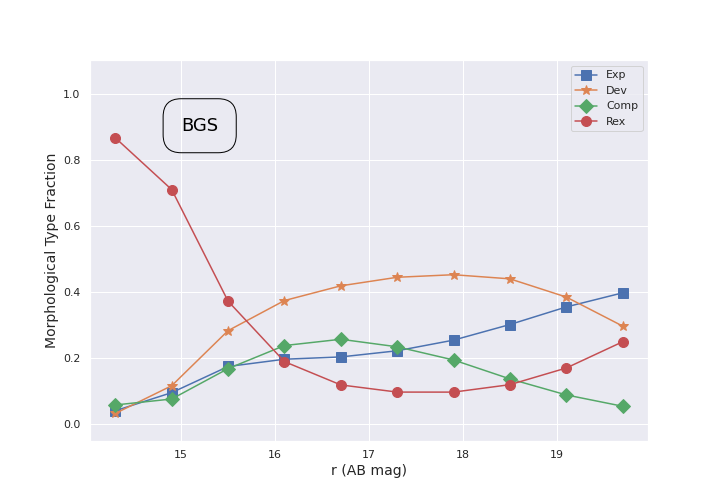
\includegraphics[width=1\linewidth]{images/gmm/bgs_morph.png}
\caption{}
\end{subfigure}
\hfill
\begin{subfigure}{.5\textwidth}
\centering
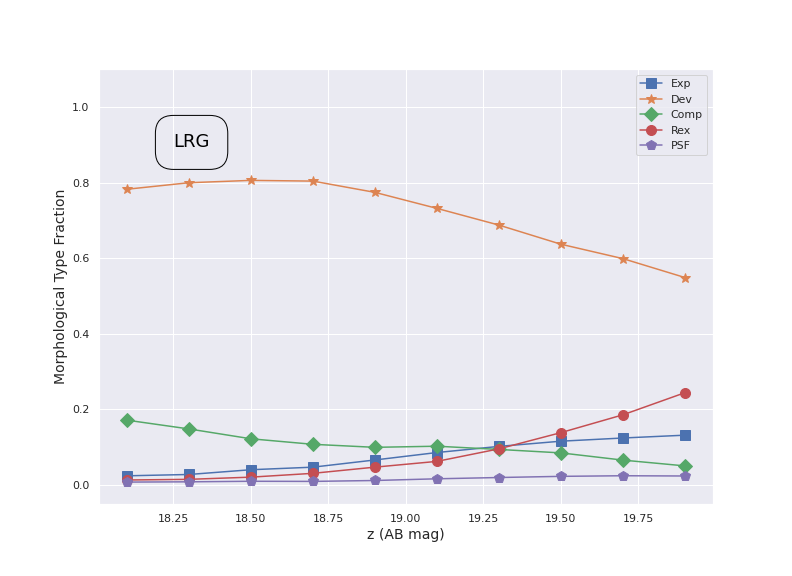
\includegraphics[width=1\linewidth]{images/gmm/lrg_morph.png}
\caption{}
\end{subfigure}
\hfill
\begin{subfigure}{.5\textwidth}
\centering
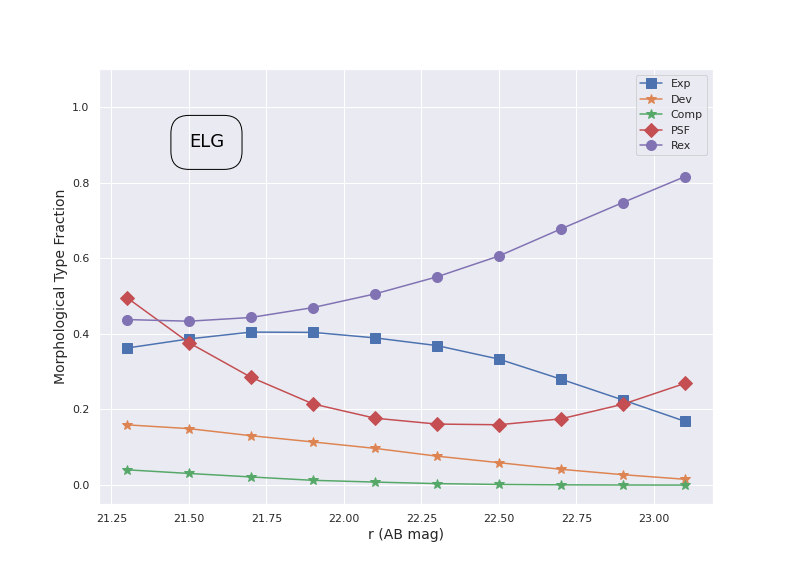
\includegraphics[width=1\linewidth]{images/gmm/elg_morph.png}
\caption{}
\end{subfigure}
\begin{subfigure}{.5\textwidth}
\centering
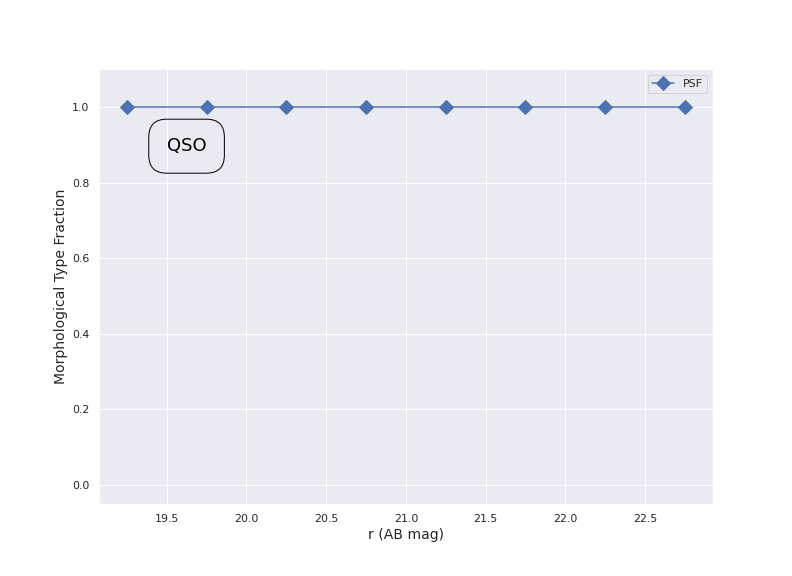
\includegraphics[width=1\linewidth]{images/gmm/qso_morph.png}
\caption{}
\end{subfigure}
\label{fig:morphfrac}
\caption{Morphological type fraction.}
\end{figure}

The features used to build the GMMs were based on the magnitudes and colors used for selection cuts for each class. GMMs were first trained on the photometry, and then the model parameters and weights were used to generate synthetic distributions of the data with the same features. The data were split into a training set used to train the model, and a validation set used to assess the performance of the model on data that were not used for training. 

Plots of the optimal number of Gaussian components determined by the BIC, as well as the 2-dimensional histograms for training and validation sets are shown in Figs. \ref{} for LRGs with deVaucoulours profiles and QSOs. The sampled data from the trained model are overlaid in green. This process was extended in a similar fashion for the remaining combinations of classes and morphologies. The contours in the histograms show the 1-, 2-, and 3-$\sigma$ contours containing 39.3\%, 86.5\%, 98.9\% of the data, respectively. 

%(Describe training/test/validation process?)

\begin{figure}
  \centering
  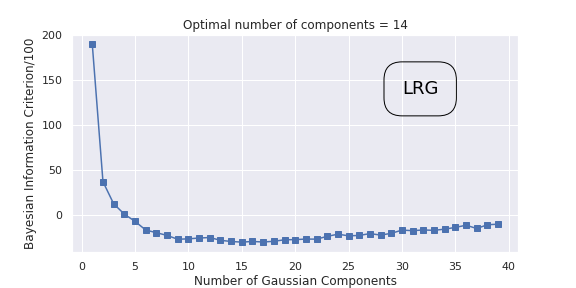
\includegraphics[width=\textwidth]{images/gmm/lrgDev_bic.png}
  \caption{LRGs.}
  \label{fig:lrg_bic}
\end{figure}

\begin{figure}
\centering
\begin{subfigure}[b]{.5\textwidth}
  \centering
  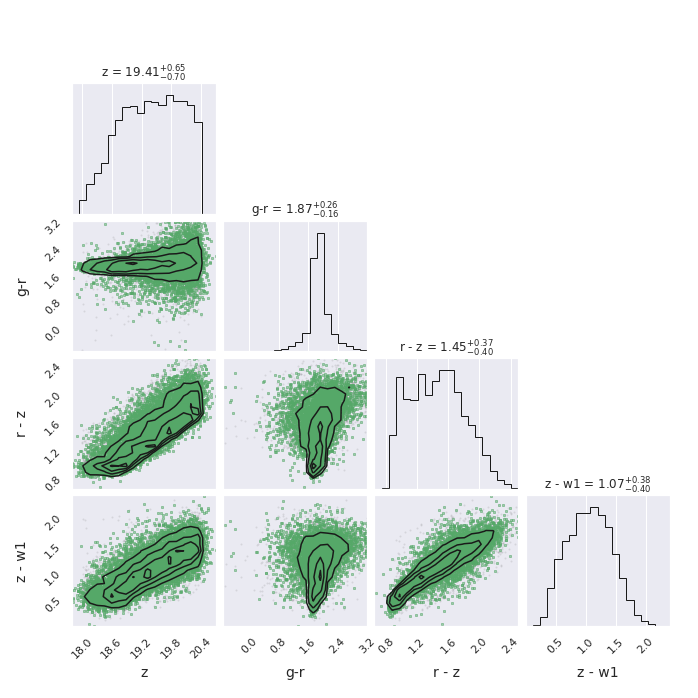
\includegraphics[width=\textwidth]{images/gmm/lrgDev_training.png}
  \caption{Training.}
  \label{fig:lrg_train}
\end{subfigure}%
\begin{subfigure}[b]{.5\textwidth}
  \centering
  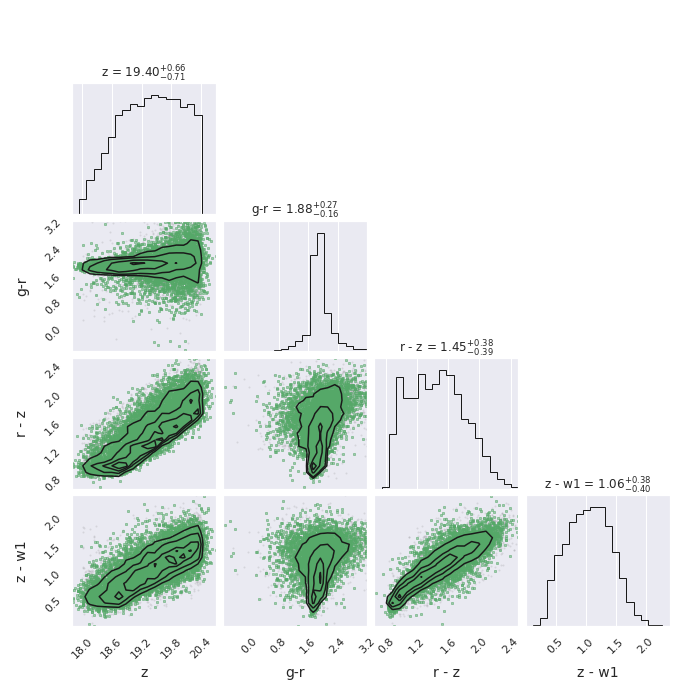
\includegraphics[width=\textwidth]{images/gmm/lrgDev_valid.png}
  \caption{Valid.}
  \label{fig:lrg_valid}
\end{subfigure}
\caption{Train/sampled/val for LRGs.}
\label{fig:lrg_gmm}
\end{figure}



\begin{figure}
  \centering
  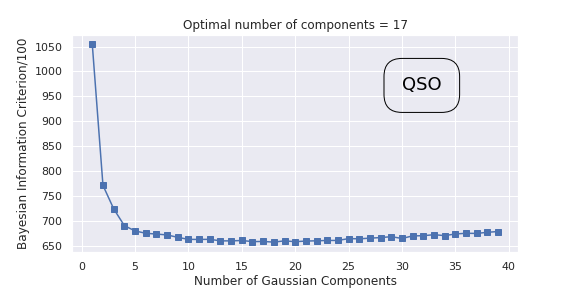
\includegraphics[width=\textwidth]{images/gmm/qso_bic.png}
  \caption{QSOs.}
  \label{fig:qso_bic}
\end{figure}

\begin{figure}
\centering
\begin{subfigure}[b]{.5\textwidth}
  \centering
  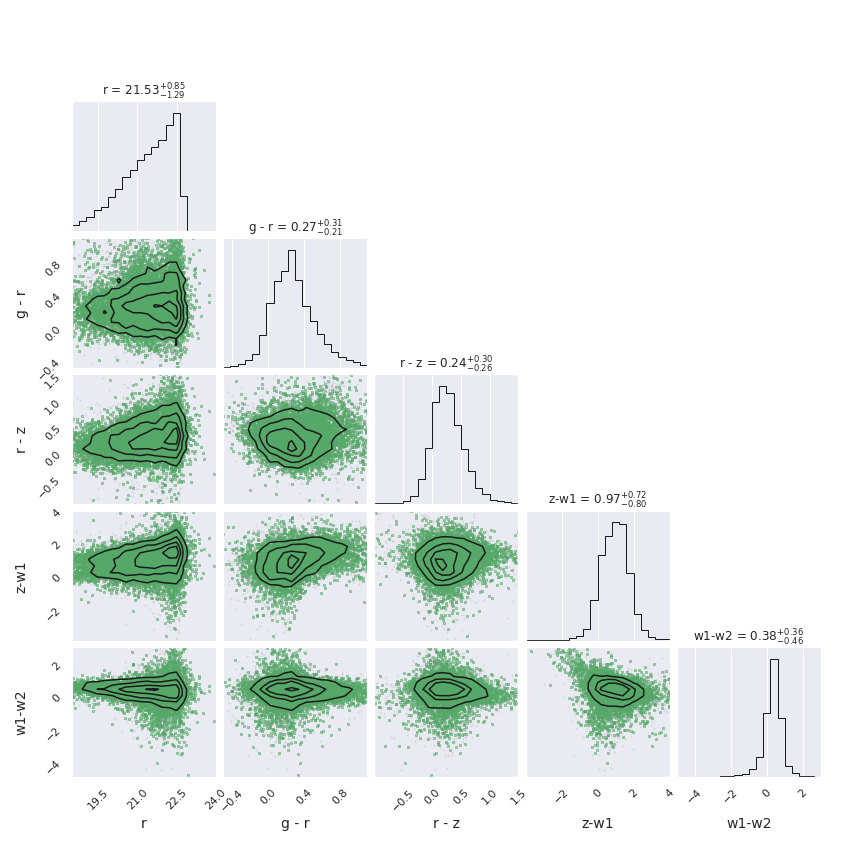
\includegraphics[width=\textwidth]{images/gmm/qso_training.png}
  \caption{Training.}
  \label{fig:qso_train}
\end{subfigure}%
\begin{subfigure}[b]{.5\textwidth}
  \centering
  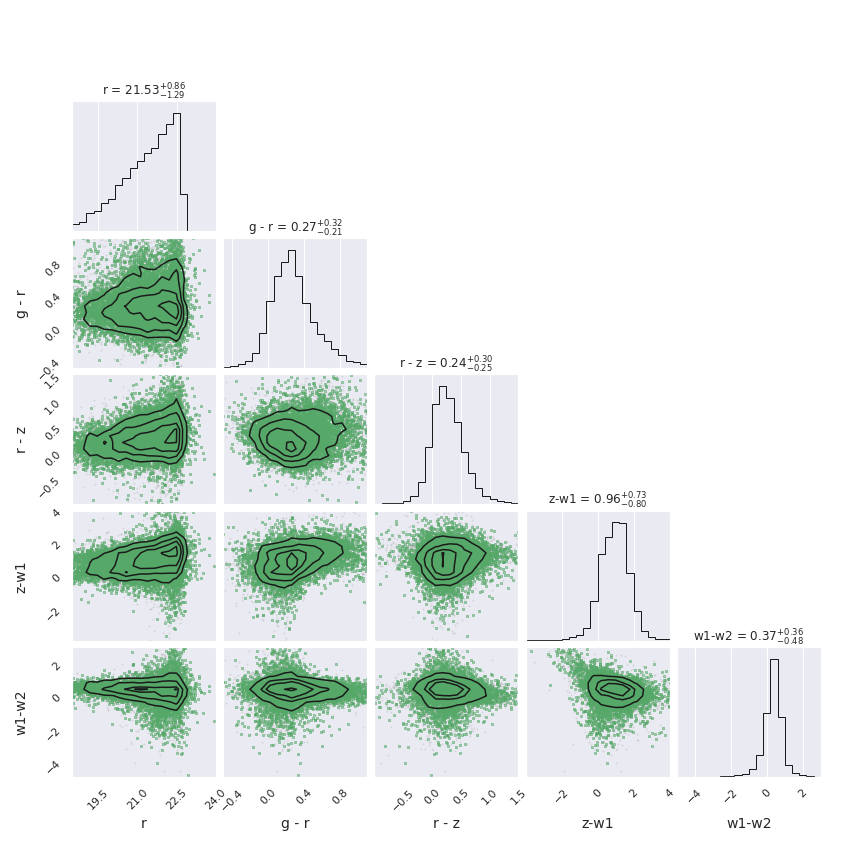
\includegraphics[width=\textwidth]{images/gmm/qso_valid.png}
  \caption{Valid.}
  \label{fig:lrg_valid}
\end{subfigure}
\caption{Train/sampled/val for QSOs.}
\label{fig:qso_gmm}
\end{figure}



\subsection{Extreme Deconvolution}

** should I add? **


%%% Local Variables: ***
%%% mode: latex ***
%%% TeX-master: "thesis.tex" ***
%%% End: ***
